\chapter{Simulação e Resultados}
\label{cap:simulacao}

\section{Metodologia}

A simulação funcional foi feita no Quartus II 9.1sp2 com o editor de formas de onda (arquivo \texttt{.vwf}). Como o circuito é combinacional, cada vetor de teste define \texttt{a\_in}, \texttt{b\_in}, \texttt{c\_in} e \texttt{op\_sel}, e o resultado é conferido após o atraso de propagação.

Os casos de teste cobrem: (i) todas as 16 operações; (ii) os seis exemplos de ADD da especificação, assim como 6 outros exemplos para as demais 15 operações; (iii) situações-limite das flags, como carry, \textit{half carry}, overflow positivo e negativo, resultado zero e resultado negativo; e (iv) o uso de \texttt{c\_in} em ADDC, SUBC, RRC e RLC.


\section{Casos de teste e resultados esperados}

As Tabelas ~\ref{tab:testes-PASS-B} a ~\ref{tab:testes-RL} lista os casos usados. Os traços indicam flags \textit{don't care} (fixadas em `0' no projeto).

\begin{longtable}{c c c c c c c c c c}
\caption{Casos de teste da operação PASS\_B.}
\label{tab:testes-PASS-B}\\
\hline
Caso & \texttt{a\_in} & \texttt{b\_in} & \texttt{c\_in} & \texttt{r\_out} & C & H & Z & V & N \\ \hline
\endfirsthead
\hline
Caso & \texttt{a\_in} & \texttt{b\_in} & \texttt{c\_in} & \texttt{r\_out} & C & H & Z & V & N \\ \hline
\endhead
1 & FF & A5 & 0 & A5 & 0 & 0 & 0 & {\footnotesize--} & 1 \\
2 & FF & 00 & 1 & 00 & 0 & 0 & 1 & {\footnotesize--} & 0 \\
3 & 12 & 7F & 0 & 7F & 0 & 0 & 0 & {\footnotesize--} & 0 \\
4 & 55 & 80 & 1 & 80 & 0 & 0 & 0 & {\footnotesize--} & 1 \\
5 & 00 & FF & 0 & FF & 0 & 0 & 0 & {\footnotesize--} & 1 \\
6 & F0 & 01 & 1 & 01 & 0 & 0 & 0 & {\footnotesize--} & 0 \\
\hline
\end{longtable}
\vspace{-0.5cm}
\fonte{Autoria propria.}

\begin{longtable}{c c c c c c c c c c}
\caption{Casos de teste da operação OR.}
\label{tab:testes-OR}\\
\hline
Caso & \texttt{a\_in} & \texttt{b\_in} & \texttt{c\_in} & \texttt{r\_out} & C & H & Z & V & N \\ \hline
\endfirsthead
\hline
Caso & \texttt{a\_in} & \texttt{b\_in} & \texttt{c\_in} & \texttt{r\_out} & C & H & Z & V & N \\ \hline
\endhead
7 & 00 & 00 & 0 & 00 & 0 & 0 & 1 & {\footnotesize--} & 0 \\
8 & F0 & 0F & 0 & FF & 0 & 0 & 0 & {\footnotesize--} & 1 \\
9 & A5 & 00 & 0 & A5 & 0 & 0 & 0 & {\footnotesize--} & 1 \\
10 & 80 & 01 & 0 & 81 & 0 & 0 & 0 & {\footnotesize--} & 1 \\
11 & 55 & AA & 0 & FF & 0 & 0 & 0 & {\footnotesize--} & 1 \\
12 & 0F & 30 & 1 & 3F & 0 & 0 & 0 & {\footnotesize--} & 0 \\
\hline
\end{longtable}
\vspace{-0.5cm}
\fonte{Autoria propria.}

\begin{longtable}{c c c c c c c c c c}
\caption{Casos de teste da operação XOR.}
\label{tab:testes-XOR}\\
\hline
Caso & \texttt{a\_in} & \texttt{b\_in} & \texttt{c\_in} & \texttt{r\_out} & C & H & Z & V & N \\ \hline
\endfirsthead
\hline
Caso & \texttt{a\_in} & \texttt{b\_in} & \texttt{c\_in} & \texttt{r\_out} & C & H & Z & V & N \\ \hline
\endhead
13 & FF & FF & 0 & 00 & 0 & 0 & 1 & {\footnotesize--} & 0 \\
14 & AA & 55 & 0 & FF & 0 & 0 & 0 & {\footnotesize--} & 1 \\
15 & F0 & 0F & 0 & FF & 0 & 0 & 0 & {\footnotesize--} & 1 \\
16 & B5 & 4C & 0 & F9 & 0 & 0 & 0 & {\footnotesize--} & 1 \\
17 & 00 & 00 & 0 & 00 & 0 & 0 & 1 & {\footnotesize--} & 0 \\
18 & 80 & 80 & 1 & 00 & 0 & 0 & 1 & {\footnotesize--} & 0 \\
\hline
\end{longtable}
\vspace{-0.5cm}
\fonte{Autoria propria.}

\begin{longtable}{c c c c c c c c c c}
\caption{Casos de teste da operação AND.}
\label{tab:testes-AND}\\
\hline
Caso & \texttt{a\_in} & \texttt{b\_in} & \texttt{c\_in} & \texttt{r\_out} & C & H & Z & V & N \\ \hline
\endfirsthead
\hline
Caso & \texttt{a\_in} & \texttt{b\_in} & \texttt{c\_in} & \texttt{r\_out} & C & H & Z & V & N \\ \hline
\endhead
19 & 0F & F0 & 0 & 00 & 0 & 0 & 1 & {\footnotesize--} & 0 \\
20 & FF & FF & 0 & FF & 0 & 0 & 0 & {\footnotesize--} & 1 \\
21 & F0 & 3C & 0 & 30 & 0 & 0 & 0 & {\footnotesize--} & 0 \\
22 & B5 & 4C & 0 & 04 & 0 & 0 & 0 & {\footnotesize--} & 0 \\
23 & 80 & FF & 0 & 80 & 0 & 0 & 0 & {\footnotesize--} & 1 \\
24 & 55 & AA & 1 & 00 & 0 & 0 & 1 & {\footnotesize--} & 0 \\
\hline
\end{longtable}
\vspace{-0.5cm}
\fonte{Autoria propria.}

\begin{longtable}{c c c c c c c c c c}
\caption{Casos de teste da operação ADDC.}
\label{tab:testes-ADDC}\\
\hline
Caso & \texttt{a\_in} & \texttt{b\_in} & \texttt{c\_in} & \texttt{r\_out} & C & H & Z & V & N \\ \hline
\endfirsthead
\hline
Caso & \texttt{a\_in} & \texttt{b\_in} & \texttt{c\_in} & \texttt{r\_out} & C & H & Z & V & N \\ \hline
\endhead
25 & 0F & 01 & 0 & 10 & 0 & 1 & 0 & 0 & 0 \\
26 & 0F & 01 & 1 & 11 & 0 & 1 & 0 & 0 & 0 \\
27 & FF & 00 & 1 & 00 & 1 & 1 & 1 & 0 & 0 \\
28 & 7F & 00 & 1 & 80 & 0 & 1 & 0 & 1 & 1 \\
29 & FF & FF & 1 & FF & 1 & 1 & 0 & 0 & 1 \\
30 & 80 & 80 & 1 & 01 & 1 & 0 & 0 & 1 & 0 \\
\hline
\end{longtable}
\vspace{-0.5cm}
\fonte{Autoria propria.}

\begin{longtable}{c c c c c c c c c c}
\caption{Casos de teste da operação ADD.}
\label{tab:testes-ADD}\\
\hline
Caso & \texttt{a\_in} & \texttt{b\_in} & \texttt{c\_in} & \texttt{r\_out} & C & H & Z & V & N \\ \hline
\endfirsthead
\hline
Caso & \texttt{a\_in} & \texttt{b\_in} & \texttt{c\_in} & \texttt{r\_out} & C & H & Z & V & N \\ \hline
\endhead
31 & 37 & 10 & 0 & 47 & 0 & 0 & 0 & 0 & 0 \\
32 & 37 & 19 & 0 & 50 & 0 & 1 & 0 & 0 & 0 \\
33 & 77 & 70 & 0 & E7 & 0 & 0 & 0 & 1 & 1 \\
34 & 77 & 89 & 0 & 00 & 1 & 1 & 1 & 0 & 0 \\
35 & 80 & 80 & 0 & 00 & 1 & 0 & 1 & 1 & 0 \\
36 & C7 & D0 & 0 & 97 & 1 & 0 & 0 & 0 & 1 \\
\hline
\end{longtable}
\vspace{-0.5cm}
\fonte{Autoria propria.}

\begin{longtable}{c c c c c c c c c c}
\caption{Casos de teste da operação SUBC.}
\label{tab:testes-SUBC}\\
\hline
Caso & \texttt{a\_in} & \texttt{b\_in} & \texttt{c\_in} & \texttt{r\_out} & C & H & Z & V & N \\ \hline
\endfirsthead
\hline
Caso & \texttt{a\_in} & \texttt{b\_in} & \texttt{c\_in} & \texttt{r\_out} & C & H & Z & V & N \\ \hline
\endhead
37 & 10 & 0F & 1 & 00 & 0 & 1 & 1 & 0 & 0 \\
38 & 10 & 0F & 0 & 01 & 0 & 1 & 0 & 0 & 0 \\
39 & 00 & 00 & 1 & FF & 1 & 1 & 0 & 0 & 1 \\
40 & 80 & 00 & 1 & 7F & 0 & 1 & 0 & 1 & 0 \\
41 & 50 & B0 & 0 & A0 & 1 & 0 & 0 & 1 & 1 \\
42 & 05 & 05 & 0 & 00 & 0 & 0 & 1 & 0 & 0 \\
\hline
\end{longtable}
\vspace{-0.5cm}
\fonte{Autoria propria.}

\begin{longtable}{c c c c c c c c c c}
\caption{Casos de teste da operação SUB.}
\label{tab:testes-SUB}\\
\hline
Caso & \texttt{a\_in} & \texttt{b\_in} & \texttt{c\_in} & \texttt{r\_out} & C & H & Z & V & N \\ \hline
\endfirsthead
\hline
Caso & \texttt{a\_in} & \texttt{b\_in} & \texttt{c\_in} & \texttt{r\_out} & C & H & Z & V & N \\ \hline
\endhead
43 & 10 & 01 & 0 & 0F & 0 & 1 & 0 & 0 & 0 \\
44 & 05 & 05 & 0 & 00 & 0 & 0 & 1 & 0 & 0 \\
45 & 00 & 01 & 0 & FF & 1 & 1 & 0 & 0 & 1 \\
46 & 80 & 01 & 0 & 7F & 0 & 1 & 0 & 1 & 0 \\
47 & 50 & B0 & 0 & A0 & 1 & 0 & 0 & 1 & 1 \\
48 & 10 & 01 & 1 & 0F & 0 & 1 & 0 & 0 & 0 \\
\hline
\end{longtable}
\vspace{-0.5cm}
\fonte{Autoria propria.}

\begin{longtable}{c c c c c c c c c c}
\caption{Casos de teste da operação NOT.}
\label{tab:testes-NOT}\\
\hline
Caso & \texttt{a\_in} & \texttt{b\_in} & \texttt{c\_in} & \texttt{r\_out} & C & H & Z & V & N \\ \hline
\endfirsthead
\hline
Caso & \texttt{a\_in} & \texttt{b\_in} & \texttt{c\_in} & \texttt{r\_out} & C & H & Z & V & N \\ \hline
\endhead
49 & 0F & 00 & 0 & F0 & 0 & {\footnotesize--} & 0 & {\footnotesize--} & 1 \\
50 & FF & 00 & 0 & 00 & 0 & {\footnotesize--} & 1 & {\footnotesize--} & 0 \\
51 & 00 & 00 & 0 & FF & 0 & {\footnotesize--} & 0 & {\footnotesize--} & 1 \\
52 & AA & 55 & 1 & 55 & 0 & {\footnotesize--} & 0 & {\footnotesize--} & 0 \\
53 & 80 & 00 & 0 & 7F & 0 & {\footnotesize--} & 0 & {\footnotesize--} & 0 \\
54 & 7F & 00 & 0 & 80 & 0 & {\footnotesize--} & 0 & {\footnotesize--} & 1 \\
\hline
\end{longtable}
\vspace{-0.5cm}
\fonte{Autoria propria.}

\begin{longtable}{c c c c c c c c c c}
\caption{Casos de teste da operação SRA.}
\label{tab:testes-SRA}\\
\hline
Caso & \texttt{a\_in} & \texttt{b\_in} & \texttt{c\_in} & \texttt{r\_out} & C & H & Z & V & N \\ \hline
\endfirsthead
\hline
Caso & \texttt{a\_in} & \texttt{b\_in} & \texttt{c\_in} & \texttt{r\_out} & C & H & Z & V & N \\ \hline
\endhead
55 & 81 & 00 & 0 & C0 & 1 & {\footnotesize--} & 0 & {\footnotesize--} & 1 \\
56 & 01 & 00 & 0 & 00 & 1 & {\footnotesize--} & 1 & {\footnotesize--} & 0 \\
57 & 7E & 00 & 0 & 3F & 0 & {\footnotesize--} & 0 & {\footnotesize--} & 0 \\
58 & 80 & 00 & 0 & C0 & 0 & {\footnotesize--} & 0 & {\footnotesize--} & 1 \\
59 & FF & 00 & 0 & FF & 1 & {\footnotesize--} & 0 & {\footnotesize--} & 1 \\
60 & 00 & 00 & 1 & 00 & 0 & {\footnotesize--} & 1 & {\footnotesize--} & 0 \\
\hline
\end{longtable}
\vspace{-0.5cm}
\fonte{Autoria propria.}

\begin{longtable}{c c c c c c c c c c}
\caption{Casos de teste da operação SRL.}
\label{tab:testes-SRL}\\
\hline
Caso & \texttt{a\_in} & \texttt{b\_in} & \texttt{c\_in} & \texttt{r\_out} & C & H & Z & V & N \\ \hline
\endfirsthead
\hline
Caso & \texttt{a\_in} & \texttt{b\_in} & \texttt{c\_in} & \texttt{r\_out} & C & H & Z & V & N \\ \hline
\endhead
61 & 81 & 00 & 0 & 40 & 1 & {\footnotesize--} & 0 & {\footnotesize--} & 0 \\
62 & 01 & 00 & 0 & 00 & 1 & {\footnotesize--} & 1 & {\footnotesize--} & 0 \\
63 & FE & 00 & 0 & 7F & 0 & {\footnotesize--} & 0 & {\footnotesize--} & 0 \\
64 & FF & 00 & 0 & 7F & 1 & {\footnotesize--} & 0 & {\footnotesize--} & 0 \\
65 & 80 & 00 & 0 & 40 & 0 & {\footnotesize--} & 0 & {\footnotesize--} & 0 \\
66 & 00 & 00 & 1 & 00 & 0 & {\footnotesize--} & 1 & {\footnotesize--} & 0 \\
\hline
\end{longtable}
\vspace{-0.5cm}
\fonte{Autoria propria.}

\begin{longtable}{c c c c c c c c c c}
\caption{Casos de teste da operação SLL.}
\label{tab:testes-SLL}\\
\hline
Caso & \texttt{a\_in} & \texttt{b\_in} & \texttt{c\_in} & \texttt{r\_out} & C & H & Z & V & N \\ \hline
\endfirsthead
\hline
Caso & \texttt{a\_in} & \texttt{b\_in} & \texttt{c\_in} & \texttt{r\_out} & C & H & Z & V & N \\ \hline
\endhead
67 & 81 & 00 & 0 & 02 & 1 & {\footnotesize--} & 0 & {\footnotesize--} & 0 \\
68 & 40 & 00 & 0 & 80 & 0 & {\footnotesize--} & 0 & {\footnotesize--} & 1 \\
69 & 01 & 00 & 0 & 02 & 0 & {\footnotesize--} & 0 & {\footnotesize--} & 0 \\
70 & FF & 00 & 0 & FE & 1 & {\footnotesize--} & 0 & {\footnotesize--} & 1 \\
71 & 80 & 00 & 0 & 00 & 1 & {\footnotesize--} & 1 & {\footnotesize--} & 0 \\
72 & 00 & 00 & 1 & 00 & 0 & {\footnotesize--} & 1 & {\footnotesize--} & 0 \\
\hline
\end{longtable}
\vspace{-0.5cm}
\fonte{Autoria propria.}

\begin{longtable}{c c c c c c c c c c}
\caption{Casos de teste da operação RRC.}
\label{tab:testes-RRC}\\
\hline
Caso & \texttt{a\_in} & \texttt{b\_in} & \texttt{c\_in} & \texttt{r\_out} & C & H & Z & V & N \\ \hline
\endfirsthead
\hline
Caso & \texttt{a\_in} & \texttt{b\_in} & \texttt{c\_in} & \texttt{r\_out} & C & H & Z & V & N \\ \hline
\endhead
73 & 01 & 00 & 1 & 80 & 1 & {\footnotesize--} & 0 & {\footnotesize--} & 1 \\
74 & 01 & 00 & 0 & 00 & 1 & {\footnotesize--} & 1 & {\footnotesize--} & 0 \\
75 & 00 & 00 & 1 & 80 & 0 & {\footnotesize--} & 0 & {\footnotesize--} & 1 \\
76 & FF & 00 & 0 & 7F & 1 & {\footnotesize--} & 0 & {\footnotesize--} & 0 \\
77 & 80 & 00 & 1 & C0 & 0 & {\footnotesize--} & 0 & {\footnotesize--} & 1 \\
78 & A5 & 00 & 0 & 52 & 1 & {\footnotesize--} & 0 & {\footnotesize--} & 0 \\
\hline
\end{longtable}
\vspace{-0.5cm}
\fonte{Autoria propria.}

\begin{longtable}{c c c c c c c c c c}
\caption{Casos de teste da operação RLC.}
\label{tab:testes-RLC}\\
\hline
Caso & \texttt{a\_in} & \texttt{b\_in} & \texttt{c\_in} & \texttt{r\_out} & C & H & Z & V & N \\ \hline
\endfirsthead
\hline
Caso & \texttt{a\_in} & \texttt{b\_in} & \texttt{c\_in} & \texttt{r\_out} & C & H & Z & V & N \\ \hline
\endhead
79 & 80 & 00 & 1 & 01 & 1 & {\footnotesize--} & 0 & {\footnotesize--} & 0 \\
80 & 80 & 00 & 0 & 00 & 1 & {\footnotesize--} & 1 & {\footnotesize--} & 0 \\
81 & 00 & 00 & 1 & 01 & 0 & {\footnotesize--} & 0 & {\footnotesize--} & 0 \\
82 & FF & 00 & 0 & FE & 1 & {\footnotesize--} & 0 & {\footnotesize--} & 1 \\
83 & 01 & 00 & 1 & 03 & 0 & {\footnotesize--} & 0 & {\footnotesize--} & 0 \\
84 & 5A & 00 & 0 & B4 & 0 & {\footnotesize--} & 0 & {\footnotesize--} & 1 \\
\hline
\end{longtable}
\vspace{-0.5cm}
\fonte{Autoria propria.}

\begin{longtable}{c c c c c c c c c c}
\caption{Casos de teste da operação RR.}
\label{tab:testes-RR}\\
\hline
Caso & \texttt{a\_in} & \texttt{b\_in} & \texttt{c\_in} & \texttt{r\_out} & C & H & Z & V & N \\ \hline
\endfirsthead
\hline
Caso & \texttt{a\_in} & \texttt{b\_in} & \texttt{c\_in} & \texttt{r\_out} & C & H & Z & V & N \\ \hline
\endhead
85 & 01 & 00 & 0 & 80 & 1 & {\footnotesize--} & 0 & {\footnotesize--} & 1 \\
86 & 02 & 00 & 0 & 01 & 0 & {\footnotesize--} & 0 & {\footnotesize--} & 0 \\
87 & 80 & 00 & 1 & 40 & 0 & {\footnotesize--} & 0 & {\footnotesize--} & 0 \\
88 & FF & 00 & 0 & FF & 1 & {\footnotesize--} & 0 & {\footnotesize--} & 1 \\
89 & A5 & 00 & 0 & D2 & 1 & {\footnotesize--} & 0 & {\footnotesize--} & 1 \\
90 & 00 & 00 & 1 & 00 & 0 & {\footnotesize--} & 1 & {\footnotesize--} & 0 \\
\hline
\end{longtable}
\vspace{-0.5cm}
\fonte{Autoria propria.}

\begin{longtable}{c c c c c c c c c c}
\caption{Casos de teste da operação RL.}
\label{tab:testes-RL}\\
\hline
Caso & \texttt{a\_in} & \texttt{b\_in} & \texttt{c\_in} & \texttt{r\_out} & C & H & Z & V & N \\ \hline
\endfirsthead
\hline
Caso & \texttt{a\_in} & \texttt{b\_in} & \texttt{c\_in} & \texttt{r\_out} & C & H & Z & V & N \\ \hline
\endhead
91 & 80 & 00 & 0 & 01 & 1 & {\footnotesize--} & 0 & {\footnotesize--} & 0 \\
92 & 40 & 00 & 0 & 80 & 0 & {\footnotesize--} & 0 & {\footnotesize--} & 1 \\
93 & 01 & 00 & 1 & 02 & 0 & {\footnotesize--} & 0 & {\footnotesize--} & 0 \\
94 & FF & 00 & 0 & FF & 1 & {\footnotesize--} & 0 & {\footnotesize--} & 1 \\
95 & A5 & 00 & 0 & 4B & 1 & {\footnotesize--} & 0 & {\footnotesize--} & 0 \\
96 & 00 & 00 & 1 & 00 & 0 & {\footnotesize--} & 1 & {\footnotesize--} & 0 \\
\hline
\end{longtable}
\vspace{-0.5cm}
\fonte{Autoria propria.}


\clearpage
\section{Formas de ondas}

\begin{figure}[!htb]
  \centering
  \caption{Simulação funcional da operação PASS\_B (\texttt{op\_sel = 0000}).}
  \label{fig:sim-pass-b}
  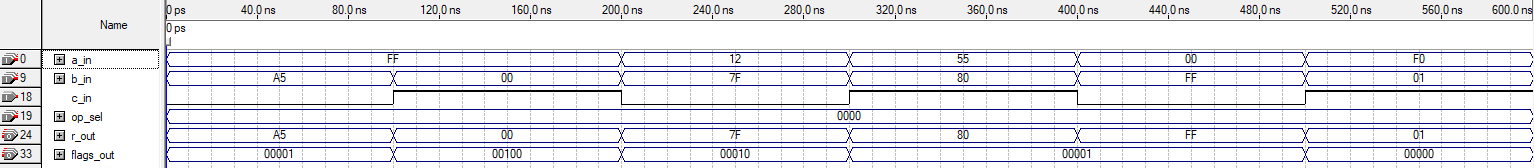
\includegraphics[width=\textwidth]{image/PASS_B.png}
  \fonte{Autoria propria (Quartus II 9.1sp2).}
\end{figure}

\begin{figure}[!htb]
  \centering
  \caption{Simulação funcional da operação OR (\texttt{op\_sel = 0001}).}
  \label{fig:sim-or}
  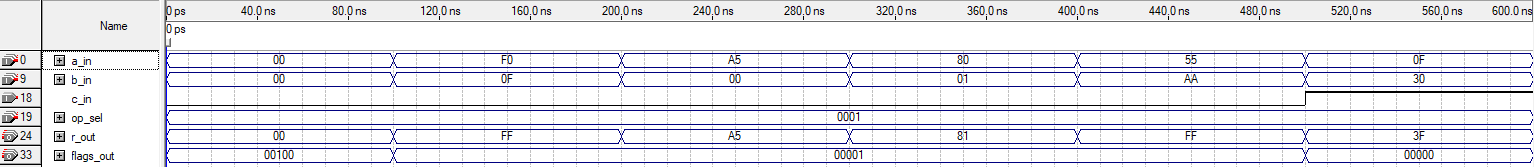
\includegraphics[width=\textwidth]{image/OR.png}
  \fonte{Autoria propria (Quartus II 9.1sp2).}
\end{figure}

\begin{figure}[!htb]
  \centering
  \caption{Simulação funcional da operação XOR (\texttt{op\_sel = 0010}).}
  \label{fig:sim-xor}
  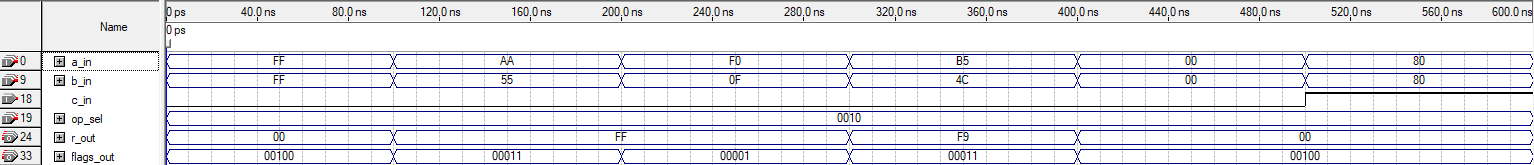
\includegraphics[width=\textwidth]{image/XOR.png}
  \fonte{Autoria propria (Quartus II 9.1sp2).}
\end{figure}

\begin{figure}[!htb]
  \centering
  \caption{Simulação funcional da operação AND (\texttt{op\_sel = 0011}).}
  \label{fig:sim-and}
  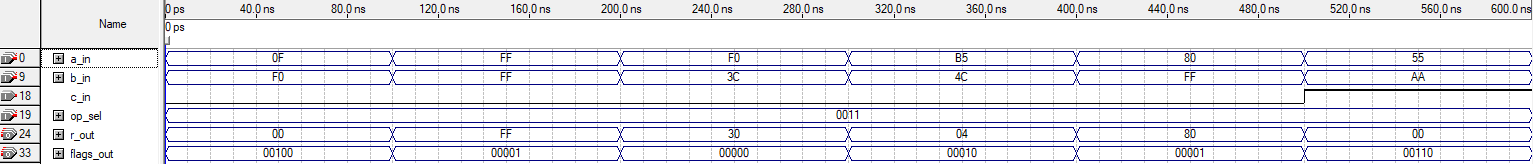
\includegraphics[width=\textwidth]{image/AND.png}
  \fonte{Autoria propria (Quartus II 9.1sp2).}
\end{figure}

\begin{figure}[!htb]
  \centering
  \caption{Simulação funcional da operação ADDC (\texttt{op\_sel = 0100}).}
  \label{fig:sim-addc}
  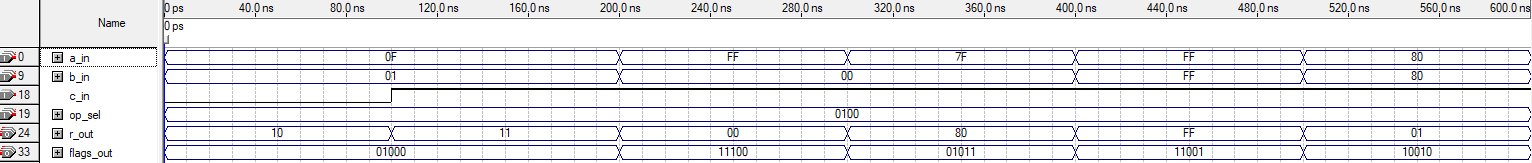
\includegraphics[width=\textwidth]{image/ADDC.png}
  \fonte{Autoria propria (Quartus II 9.1sp2).}
\end{figure}

\begin{figure}[!htb]
  \centering
  \caption{Simulação funcional da operação ADD (\texttt{op\_sel = 0101}).}
  \label{fig:sim-add}
  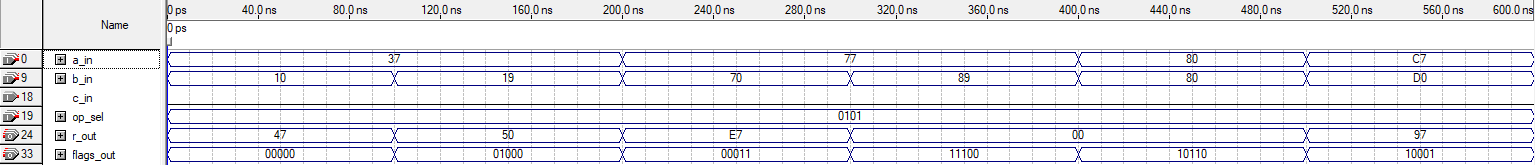
\includegraphics[width=\textwidth]{image/ADD.png}
  \fonte{Autoria propria (Quartus II 9.1sp2).}
\end{figure}

\begin{figure}[!htb]
  \centering
  \caption{Simulação funcional da operação SUBC (\texttt{op\_sel = 0110}).}
  \label{fig:sim-subc}
  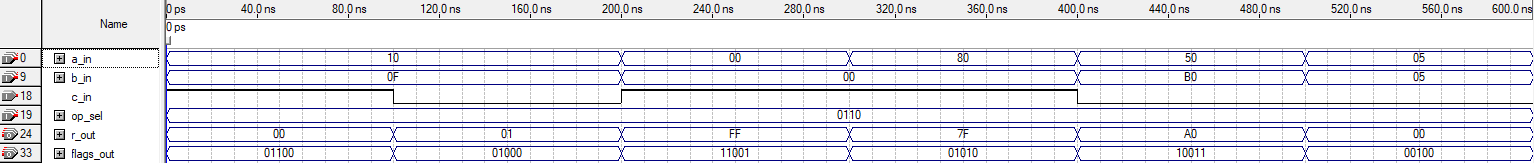
\includegraphics[width=\textwidth]{image/SUBC.png}
  \fonte{Autoria propria (Quartus II 9.1sp2).}
\end{figure}

\begin{figure}[!htb]
  \centering
  \caption{Simulação funcional da operação SUB (\texttt{op\_sel = 0111}).}
  \label{fig:sim-sub}
  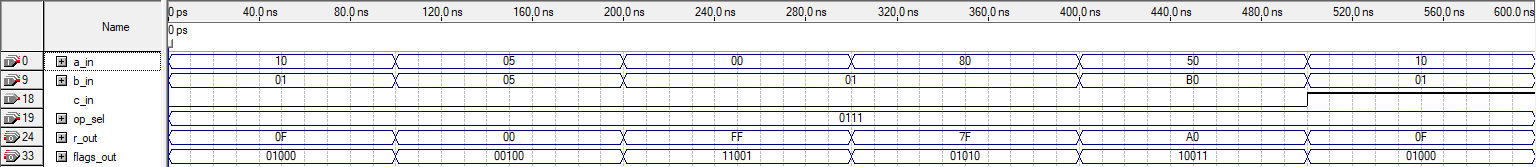
\includegraphics[width=\textwidth]{image/SUB.png}
  \fonte{Autoria propria (Quartus II 9.1sp2).}
\end{figure}

\begin{figure}[!htb]
  \centering
  \caption{Simulação funcional da operação NOT (\texttt{op\_sel = 1000}).}
  \label{fig:sim-not}
  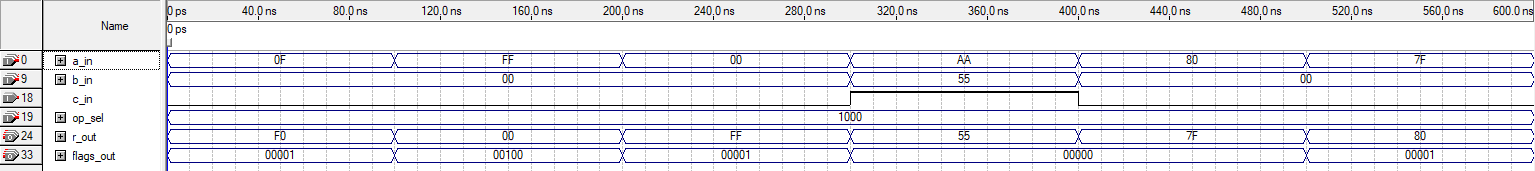
\includegraphics[width=\textwidth]{image/NOT.png}
  \fonte{Autoria propria (Quartus II 9.1sp2).}
\end{figure}

\begin{figure}[!htb]
  \centering
  \caption{Simulação funcional da operação SRA (\texttt{op\_sel = 1001}).}
  \label{fig:sim-sra}
  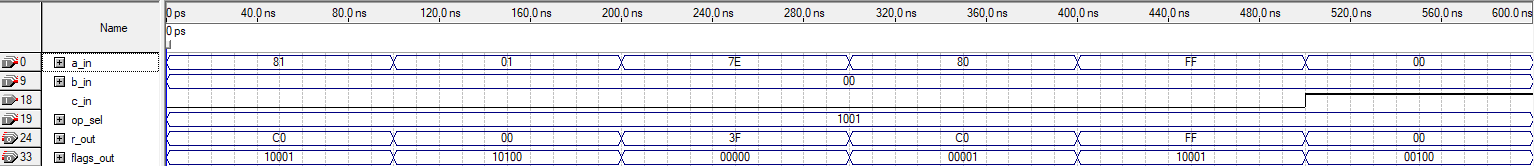
\includegraphics[width=\textwidth]{image/SRA.png}
  \fonte{Autoria propria (Quartus II 9.1sp2).}
\end{figure}

\begin{figure}[!htb]
  \centering
  \caption{Simulação funcional da operação SRL (\texttt{op\_sel = 1010}).}
  \label{fig:sim-srl}
  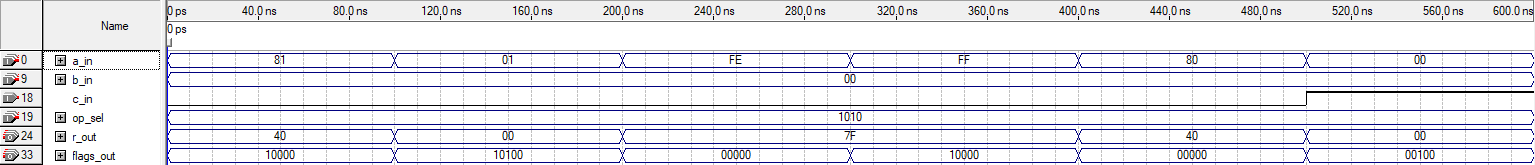
\includegraphics[width=\textwidth]{image/SRL.png}
  \fonte{Autoria propria (Quartus II 9.1sp2).}
\end{figure}

\begin{figure}[!htb]
  \centering
  \caption{Simulação funcional da operação SLL (\texttt{op\_sel = 1011}).}
  \label{fig:sim-sll}
  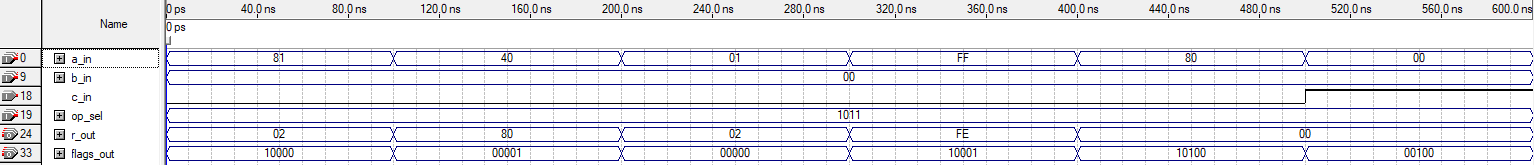
\includegraphics[width=\textwidth]{image/SLL.png}
  \fonte{Autoria propria (Quartus II 9.1sp2).}
\end{figure}

\begin{figure}[!htb]
  \centering
  \caption{Simulação funcional da operação RRC (\texttt{op\_sel = 1100}).}
  \label{fig:sim-rrc}
  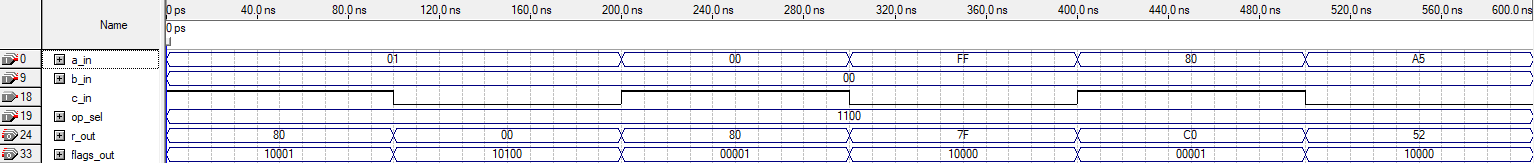
\includegraphics[width=\textwidth]{image/RRC.png}
  \fonte{Autoria propria (Quartus II 9.1sp2).}
\end{figure}

\begin{figure}[!htb]
  \centering
  \caption{Simulação funcional da operação RLC (\texttt{op\_sel = 1101}).}
  \label{fig:sim-rlc}
  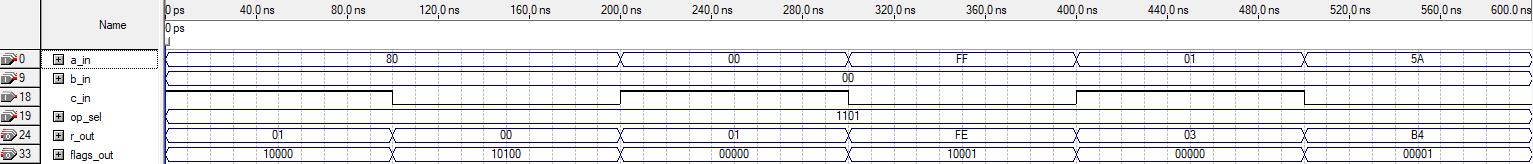
\includegraphics[width=\textwidth]{image/RLC.png}
  \fonte{Autoria propria (Quartus II 9.1sp2).}
\end{figure}

\begin{figure}[!htb]
  \centering
  \caption{Simulação funcional da operação RR (\texttt{op\_sel = 1110}).}
  \label{fig:sim-rr}
  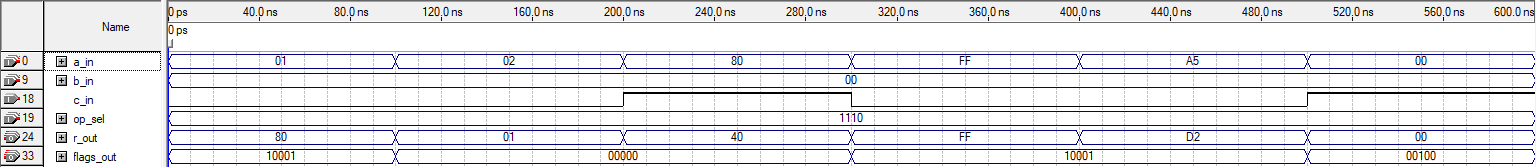
\includegraphics[width=\textwidth]{image/RR.png}
  \fonte{Autoria propria (Quartus II 9.1sp2).}
\end{figure}

\begin{figure}[!htb]
  \centering
  \caption{Simulação funcional da operação RL (\texttt{op\_sel = 1111}).}
  \label{fig:sim-rl}
  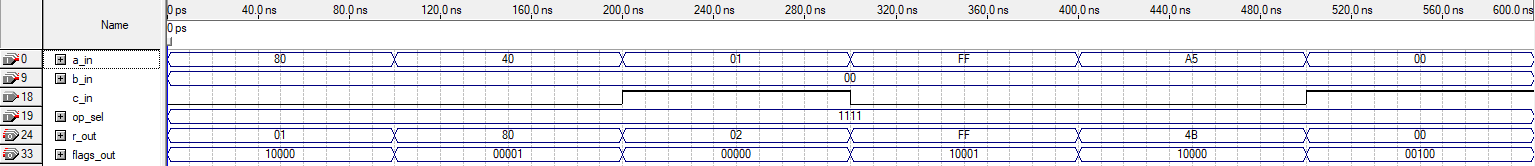
\includegraphics[width=\textwidth]{image/RL.png}
  \fonte{Autoria propria (Quartus II 9.1sp2).}
\end{figure}

\clearpage
\section{Análise dos resultados}

Os resultados foram analisados a partir dos 96 casos apresentados nas tabelas
individuais de cada operação e das formas de onda obtidas no Quartus II. Em
todos os casos, foram comparados o valor de \texttt{r\_out} e o estado das
flags C, H, Z, V e N. Essa comparação é importante porque uma operação pode
produzir o resultado numérico correto e, ainda assim, apresentar erro em uma
das flags.

\subsection{Operações lógicas}

As operações \texttt{PASS\_B}, \texttt{OR}, \texttt{XOR} e \texttt{AND}
apresentaram o comportamento esperado para todas as combinações testadas. Em
\texttt{PASS\_B}, o resultado acompanha diretamente \texttt{b\_in},
independentemente do valor de \texttt{a\_in} e de \texttt{c\_in}. Nas demais
operações, cada bit do resultado corresponde à aplicação da operação lógica
entre os bits de mesma posição dos operandos.

Nessas quatro operações, C e H permanecem em zero, pois não existe propagação
de carry ou borrow. A flag V também é tratada como ``don't care'' pela
especificação e foi mantida em zero na implementação. As flags Z e N foram
geradas a partir do resultado selecionado: Z é ativada somente quando
\texttt{r\_out} é igual a zero, enquanto N reproduz o bit mais significativo
do resultado. Os casos com resultados \texttt{00} e \texttt{FF} confirmam,
respectivamente, o funcionamento das flags Z e N.

\subsection{Operações de soma}

As operações \texttt{ADDC} e \texttt{ADD} confirmaram o funcionamento do
caminho aritmético compartilhado. Em \texttt{ADDC}, o valor de
\texttt{c\_in} participa da soma; em \texttt{ADD}, ele é ignorado e o carry
inicial é zero. A diferença pode ser observada nos casos em que os operandos
são iguais, mas o carry de entrada varia, como em
$0F + 01 + 0 = 10$ e $0F + 01 + 1 = 11$.

Os seis exemplos de \texttt{ADD} da especificação também foram reproduzidos.
O caso $37h + 10h = 47h$ não produz flags de exceção; $37h + 19h = 50h$
produz \textit{half carry}; e $77h + 70h = E7h$ apresenta overflow e
resultado negativo. No caso $77h + 89h = 00h$, ocorre simultaneamente carry,
\textit{half carry} e zero. Já $80h + 80h = 00h$ demonstra a ocorrência de
carry e overflow com resultado zero, enquanto $C7h + D0h = 97h$ produz carry
sem overflow. Esses casos mostram que carry e overflow representam condições
diferentes: o primeiro está relacionado ao transporte além do oitavo bit, e o
segundo à interpretação com sinal.

\subsection{Operações de subtração}

Os resultados de \texttt{SUBC} e \texttt{SUB} confirmam a implementação da
subtração por complemento de dois. O operando B é invertido e o carry inicial
é ajustado para que a soma produza a diferença desejada. Em \texttt{SUBC},
\texttt{c\_in} é incluído como empréstimo; em \texttt{SUB}, a operação é feita
sem empréstimo inicial.

Nas subtrações, C e H representam borrow, conforme a convenção adotada no
projeto. Por exemplo, $10h - 20h = F0h$ gera borrow e resultado negativo.
Também é possível observar a diferença entre borrow e overflow no caso
$80h - 01h = 7Fh$: o resultado aritmético excede o intervalo representável
com sinal, portanto V é ativada, embora o resultado binário seja positivo.
Nos casos em que os operandos são iguais, o resultado é zero, Z é ativada e
as flags de borrow permanecem inativas.

\subsection{Deslocamentos e rotações}

Nas operações \texttt{SRA}, \texttt{SRL} e \texttt{SLL}, o bit removido da
palavra é copiado para C. A operação \texttt{SRA} preserva o bit de sinal ao
preencher a posição mais significativa, enquanto \texttt{SRL} preenche essa
posição com zero. Em \texttt{SLL}, o bit menos significativo recebe zero e o
bit mais significativo deslocado é utilizado para atualizar C.

Os resultados confirmam, por exemplo, que \texttt{81h} deslocado
aritmeticamente à direita produz \texttt{C0h}, preservando o bit de sinal, ao
passo que o deslocamento lógico produz \texttt{40h}. Em todas essas operações,
H e V não são relevantes e permanecem fixadas em zero, conforme definido na
especificação.

Nas rotações com carry, \texttt{RRC} e \texttt{RLC}, o valor de
\texttt{c\_in} é inserido na palavra durante a rotação. Em \texttt{RRC}, o
bit menos significativo deslocado ocupa a posição de C e o carry de entrada
entra no bit mais significativo. Em \texttt{RLC}, ocorre o processo inverso.
Os casos com \texttt{c\_in} igual a zero e a um confirmam que essa entrada
não é apenas uma flag de controle, mas participa efetivamente do resultado.

Nas rotações \texttt{RR} e \texttt{RL}, não há carry de entrada: o bit
expulso retorna pela extremidade oposta da palavra. Assim, a rotação de
\texttt{01h} para a direita produz \texttt{80h}, enquanto a rotação de
\texttt{80h} para a esquerda produz \texttt{01h}. Esses casos também
confirmam que C recebe o bit que foi expulso.

\subsection{Avaliação geral das flags}

As flags Z e N foram consistentes em todas as classes de operação. Z foi
ativada para resultados \texttt{00h}, inclusive quando o valor zero foi
obtido por uma soma, subtração, operação lógica ou deslocamento. N acompanhou
corretamente o bit 7 de \texttt{r\_out}, permanecendo ativa para resultados
como \texttt{80h}, \texttt{A5h}, \texttt{C0h} e \texttt{FFh}.

As flags C, H e V foram avaliadas de acordo com a natureza da operação. C e H
foram utilizados nas operações aritméticas, C também registrou o bit expulso
nos deslocamentos e rotações, e V foi utilizada para indicar overflow com
sinal nas somas e subtrações. Nas operações em que a especificação não define
uma dessas flags, o valor zero evita estados indefinidos e torna a forma de
onda mais simples de interpretar.

De modo geral, a comparação entre as tabelas de resultados esperados e as
formas de onda confirma a correção funcional da ALU para as 16 operações
implementadas. Os testes também verificam as situações de limite mais
relevantes, incluindo carry, borrow, \textit{half carry}, overflow, zero,
resultado negativo e o uso do carry de entrada.
